\chapter{Juegos}
\label{cap:juegos}
En este capítulo se explican los diferentes tipos de juegos en función de las características que los hacen interesantes para la IA.
Nos centraremos en una clase especializada: juegos con búsqueda con adversarios.
Concretamente se estudian dos: el juego del Conecta-4 y el juego del Go.

\bigskip
Los juegos proporcionan una tarea estructurada en la que es muy fácil medir el éxito o el fracaso. 
En comparación con otras aplicaciones de IA, los juegos no necesitan grandes cantidades de conocimiento.

Los juegos son conocidos en IA como \textbf{problemas de búsqueda con adversarios} porque se trata de entornos competitivos en los cuales los objetivos de los agentes\footnote{En el capítulo~\ref{cap:estrategias} se definirá formalmente el término agente, pero por ahora podemos considerar un agente como un jugador de juegos.
} están en conflicto.
Estos problemas se resuelven mediante los denominados ``algoritmos de juegos'', los cuales se estudiarán en el capítulo~\ref{cap:estrategias}.

\section{Características de los juegos}
\label{sec:caracteristicas_juegos}
Este proyecto está orientado a una clase de juegos especializada: juegos de suma cero, de dos jugadores, por turnos, deterministas y de información perfecta.
Los problemas de juegos en IA pueden clasificarse según estas propiedades:
\begin{itemize}
	\item \textbf{Número de jugadores} \\
	Un juego puede ser para un jugador sin adversario (conocidos como puzzles o solitarios, por ejemplo el Puzzle-8 o el Cubo de Rubik), para dos jugadores (bipersonales) o para N jugadores.
	\item \textbf{Suma cero} \\
	Un juego de suma cero describe una situación con adversarios, en la que los valores de utilidad al final del juego, son siempre iguales y opuestos. Esto quiere decir que la ganancia o pérdida de un agente se equilibra con exactitud con las pérdidas o ganancias de los otros agentes.
Por ejemplo, si un jugador gana una partida de Ajedrez (+1), el otro jugador necesariamente pierde (-1).
	\item \textbf{Orden de los movimientos} \\
Los agentes pueden realizar sus acciones alternativamente (por turnos), al azar o incluso realizar cada agente un número determinado de acciones seguidas.
	\item \textbf{Información perfecta} \\
	En un juego con información perfecta no interviene el azar y los estados del juego son totalmente observables, es decir, los agentes tienen un conocimiento perfecto del estado actual del juego en cada momento y es el mismo para todos los agentes.
Por el contrario, en un juego con información imperfecta puede intervenir el azar y puede haber ocultación de información entre los agentes.
	\item \textbf{Determinismo} \\
	Un juego es determinista si no aparece el azar en algunas de las propiedades anteriores.
En caso contrario el juego es indeterminista o estocástico.
\end{itemize}
Teniendo esto en cuenta, los juegos a considerar son aquellos que presenten entornos deterministas, totalmente observables en los cuales hay dos agentes cuyas acciones deben alternar y en los que los valores de utilidad al final son iguales y opuestos.
Ejemplos de juegos que cumplen estas propiedades son: el ajedrez, las damas, el 3 en Raya, el Othello o Reversi y por supuesto los dos juegos que se proponen en este proyecto: el Conecta-4 y el Go.
En IA, a este tipo de juegos se les conoce como \textit{classic board-games} en la literatura anglosajona.

\section{Juegos como problemas de búsqueda con adversarios}
\label{sec:juegos_problemas_busqueda_adversario}
Un juego puede definirse formalmente como una clase de problemas de búsqueda con los siguientes elementos:
\begin{itemize}
	\item Un \textbf{estado inicial}, que incluye la situación inicial de la partida (por ejemplo la posición inicial del tablero) e identifica al jugador que mueve.
	\item Una \textbf{función sucesor}, que devuelve una lista de pares (movimiento, estado), indicando un movimiento legal y el estado resultante.
	\item Un \textbf{test terminal} que determina cuándo se termina el juego.
	A los estados donde el juego se ha terminado se les llaman estados terminales.
	\item Una \textbf{función de utilidad} (también llamada función objetivo o función de rentabilidad), que da un valor numérico a los estados terminales. Por ejemplo, +1, -1 ó 0 cuando el resultado de un juego es un triunfo, una pérdida o un empate respectivamente.
\end{itemize}
Estos elementos permiten construir un \textbf{espacio de estados} donde puedan actuar los algoritmos de búsqueda.
Los algoritmos interpretan el espacio de estados de los juegos como un  \textbf{árbol de juegos} o \textbf{árbol de búsqueda}.
Estos conceptos se definirán en detalle en el capítulo~\ref{cap:estrategias}.

El tamaño del espacio de estados permite clasificar los juegos por su complejidad.
La tabla~\ref{tab:complejidad_juegos} presenta varios juegos clásicos; para cada uno de ellos se muestra la complejidad del árbol de búsqueda en función del número de nodos que contiene y se muestra la clase de complejidad\footnote{\textit{PSPACE} es la clase de problemas resolubles en espacio polinómico. \textit{EXPTIME} es la clase de problemas resolubles en tiempo exponencial. Un problema \textit{P} es \textit{C-completo} (donde \textit{C} es la clase de complejidad del problema \textit{P}) si cualquier otro problema de la clase \textit{C} es reducible a \textit{P}.} a la que pertenece \citeref{complejidadJuegos}.
\begin{table}[!h]
\caption{Complejidad de los juegos clásicos de tablero.}
\label{tab:complejidad_juegos}	% La etiqueta debe ir justo despues de caption o dentro de él.
\begin{center}
\begin{tabular}{lcl}
\hline
\textbf{Juego} & \textbf{Tamaño del árbol de juegos} & \textbf{Clase de complejidad}\\
%\hline
3 en raya & $10^{5}$ & PSPACE-completo\\
Conecta-4 & $10^{21}$ & PSPACE\\ 
Damas & $10^{31}$ & EXPTIME-completo\\
Othello o Reversi & $10^{58}$ & PSPACE-completo\\ 
Ajedrez & $10^{123}$ & EXPTIME-completo\\ 
Go (19x19) & $10^{360}$ & EXPTIME-completo\\
\hline
\end{tabular}
\end{center}
\end{table}
% PONER EN LA INTRODUCCION
%Los juegos son un tema atractivo a estudiar para los investigadores de
%Inteligencia Artificial (IA). La naturaleza abstracta de los juegos, la facilidad
%de representar el estado de los mismos y la definición precisa de sus reglas
%hace que hayan tenido mucho interés en la comunidad de IA.

\bigskip
A continuación se presentan los juegos desarrollados en el proyecto: el Conecta-4 y el Go.

\section{El juego del Conecta-4}
\label{sec:juego_conecta4}
El \textit{Conecta-4} (también conocido como \textit{4 en línea}) es un juego para dos jugadores en el que el objetivo es ser el primero en hacer una línea de cuatro fichas consecutivas del mismo color.

Se ha considerado una versión generalizada del juego con un tablero de \textit{n} filas $\times$ \textit{m} columnas y una longitud ganadora de \textit{k} fichas; aunque las reglas del juego no se ven afectadas por estos parámetros.

\subsection{Reglas del juego}
\label{ssec:reglas_conecta4}
El juego se desarrolla en un tablero en posición vertical de 6 filas y 7 columnas.
Cada jugador dispone de fichas de un color y se turnan para soltarlas en las columnas.
Las fichas ocuparan la posiciones más bajas de las columnas. 
En cada turno sólo puede soltarse una ficha en cualquiera de las columnas siempre que la columna no esté completa.

Un jugador gana cuando consigue colocar cuatro de sus fichas en línea (horizontal, vertical o diagonal).
Si todas las columnas se llenan de fichas y ningún jugador ha conseguido conectar cuatro fichas, la partida termina en empate.



\section{El juego del Go}
\label{sec:juego_go}
El Go es un juego de mesa estratégico muy popular en Asia.
En él, dos jugadores colocan alternativamente fichas negras y blancas (llamadas \textbf{piedras})  sobre las intersecciones libres de un tablero de dimensiones 19$\times$19.
El objetivo del juego es controlar una porción más grande del tablero que el oponente.

Existen versiones del juego en tableros más pequeños (9$\times$9, 13$\times$13 ó 17$\times$17).
El tamaño más común es 19$\times$19 y es el que se usa en los torneos oficiales \citeref{InternationalGoFederation, EuropeanGoFederation}.
Aquí se ha considerado una versión generalizada del juego en un tablero de dimensiones \textit{N$\times$N}.

\bigskip
A continuación se exponen las reglas del juego, basadas en las \textit{``Reglas Tromp/Taylor''} (más conocidas como \textit{``Reglas lógicas del Go''}) que tienen las características de ser muy elegantes y concisas \citeref{reglasLogicas}.

\subsection{Reglas del juego}
\label{ssec:reglas_go}
Al inicio de la partida el tablero está vacío y se juega con $N \times N$ piedras blancas y $N \times N+1$ negras, donde $N \times N$ son las dimensiones del tablero (180 piedras blancas y 181 negras para un tablero 19$\times$19).
El jugador con las piedras negras juega primero. 
Después ambos jugadores mueven por turnos.
Un movimiento consiste en poner una piedra en una intersección vacía del tablero o bien pasar el turno. Si ambos jugadores pasan el turno consecutivamente, la partida termina.

Dos o más piedras juntas (horizontal o verticalmente) del mismo color forman un \textbf{grupo}.
Las \textbf{libertades} de una piedra o grupo son las intersecciones vacías horizontales o verticales, adyacentes a esa piedra o grupo. 
Una piedra sola en el medio del tablero tiene cuatro libertades, una piedra en el borde tiene tres libertades y una piedra en la esquina tiene dos.

Una piedra o grupo de piedras se captura y retira del tablero de juego si no tiene libertades, esto es, si se encuentra completamente rodeada de piedras del color contrario.
Las piedras capturadas no pueden volver a jugarse durante la partida.

En principio está permitido jugar en cualquier punto del tablero (incluidos los bordes y las esquinas), pero existen dos movimientos prohibidos: el \textbf{suicidio} y la \textbf{situación de \textit{Ko}}.
\begin{itemize}
	\item \textbf{Suicidio} \\
	Está prohibido ubicar una piedra en una posición que no captura ninguna otra y deja a su propia piedra o grupo sin libertades. En la figura~\ref{fig:go_suicidio} se aprecia esta situación, mientras que la figura~\ref{fig:go_no_suicidio} no representa una situación de suicidio.
\begin{figure}[t]
	\centering
	% Primera imagen
	\begin{minipage}[t]{0.4\linewidth}
		\centering
		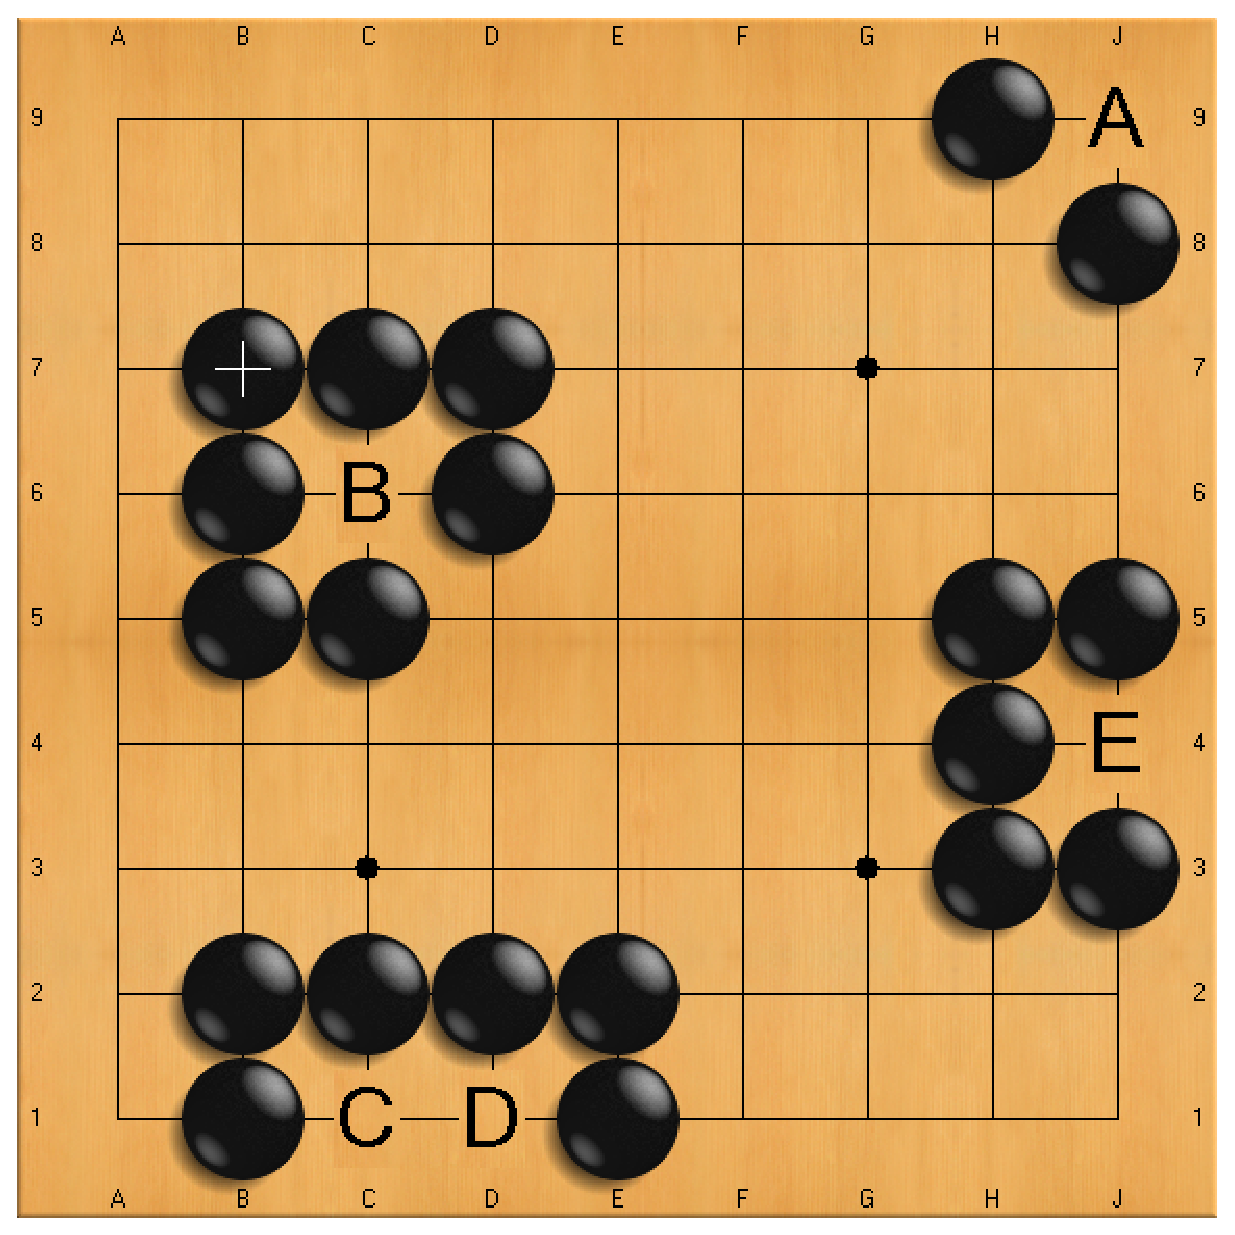
\includegraphics[scale=0.2]{contenido/cap2/imagenes/suicidio.eps}
		\caption[Situación de suicidio en el Go]{Situación de suicidio. Blancas no pueden mover en A, B o E.}
		\label{fig:go_suicidio}
	\end{minipage}
	\hspace{1cm}
	% Segunda imagen
	\begin{minipage}[t]{0.4\linewidth}
		\centering
		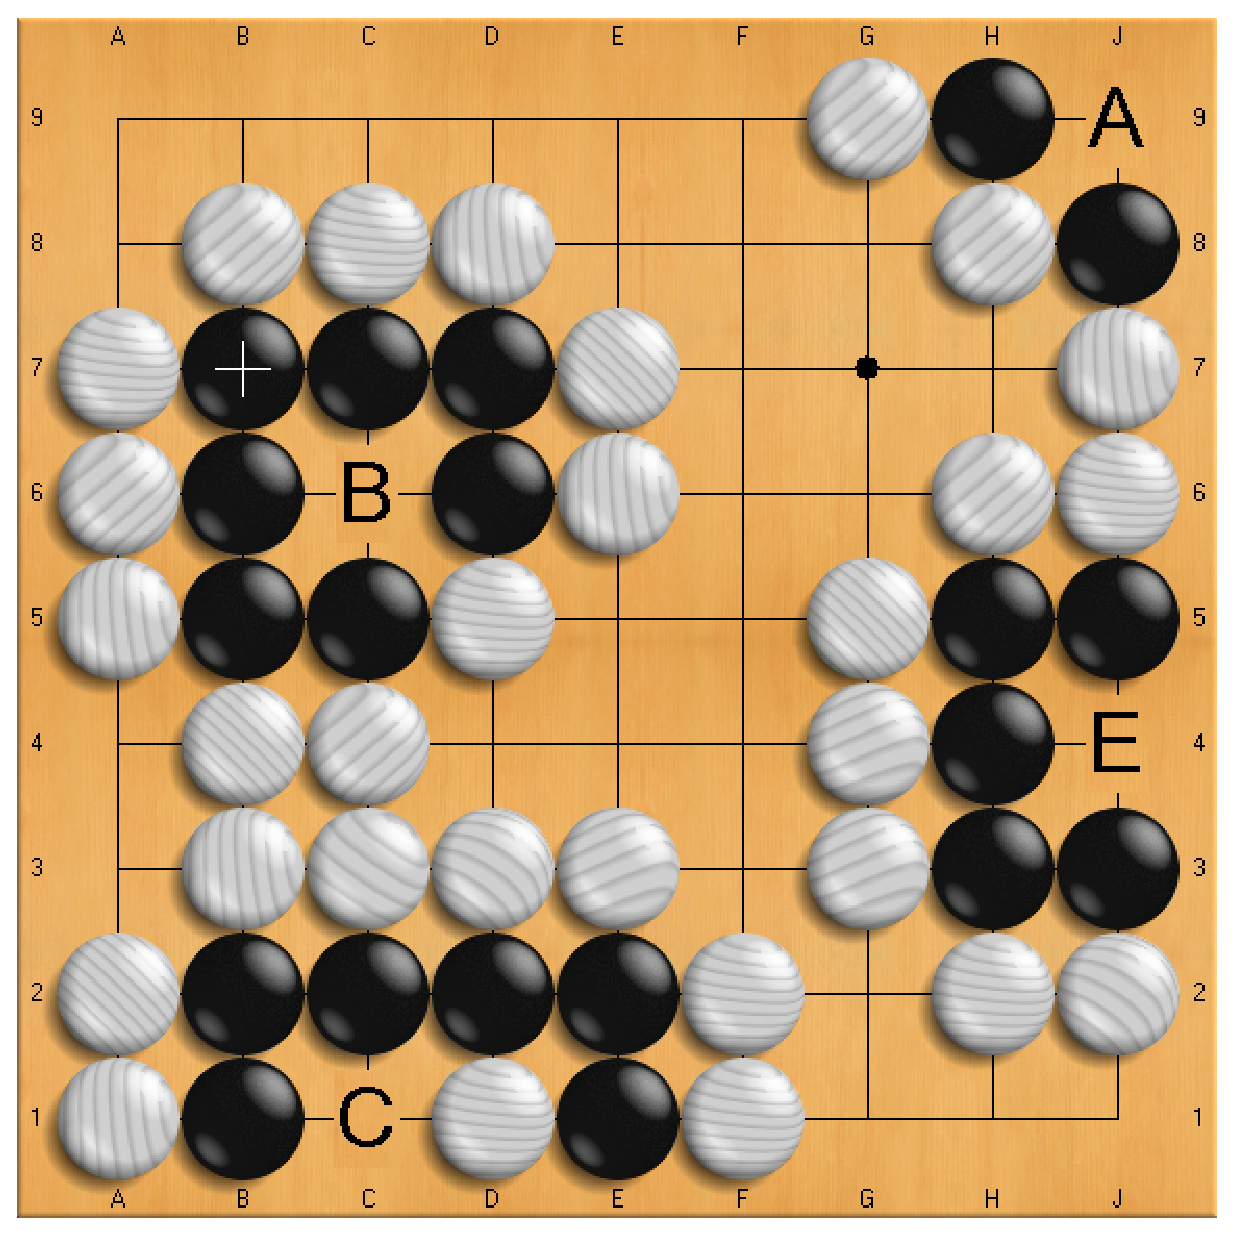
\includegraphics[scale=0.2]{contenido/cap2/imagenes/no_suicidio.eps}
		\caption[Situación de captura en el Go]{Blancas pueden mover en A, B, C o E, pues ha rodeado completamente al enemigo.}
		\label{fig:go_no_suicidio}
	\end{minipage}
\end{figure}
	\item \textbf{La regla del \textit{Ko}} \\
	La regla del \textit{Ko} evita que las posiciones de las piedras en el tablero se repitan en dos turnos diferentes.
Los tableros de la figura~\ref{fig:go_ko} reflejan esta situación.
Si un jugador captura una piedra en situación de \textit{Ko}, otro jugador no puede recapturar la misma piedra inmediatamente; ha de hacer otra jugada antes de recapturar.
Se trata de evitar una situación de infinitud.
\begin{figure}[t]
	\centering
	% Primera imagen
	\begin{minipage}[t]{0.4\linewidth}
		\centering
		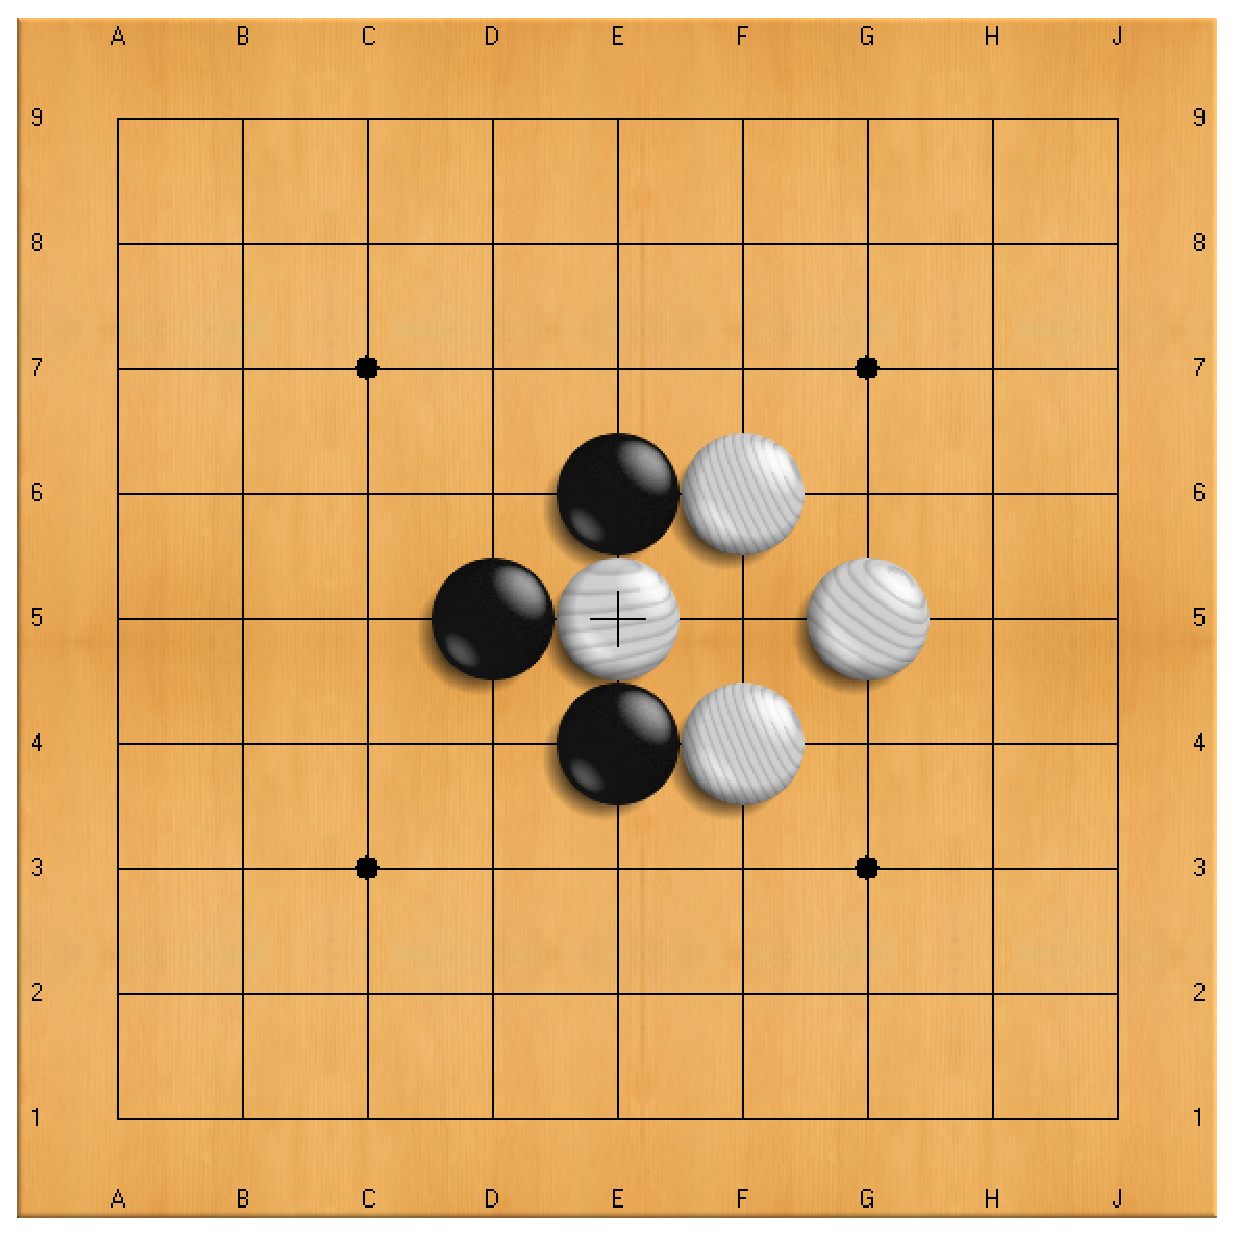
\includegraphics[scale=0.2]{contenido/cap2/imagenes/ko1.eps}
	\end{minipage}
	\hspace{1cm}
	% Segunda imagen
	\begin{minipage}[t]{0.4\linewidth}
		\centering
		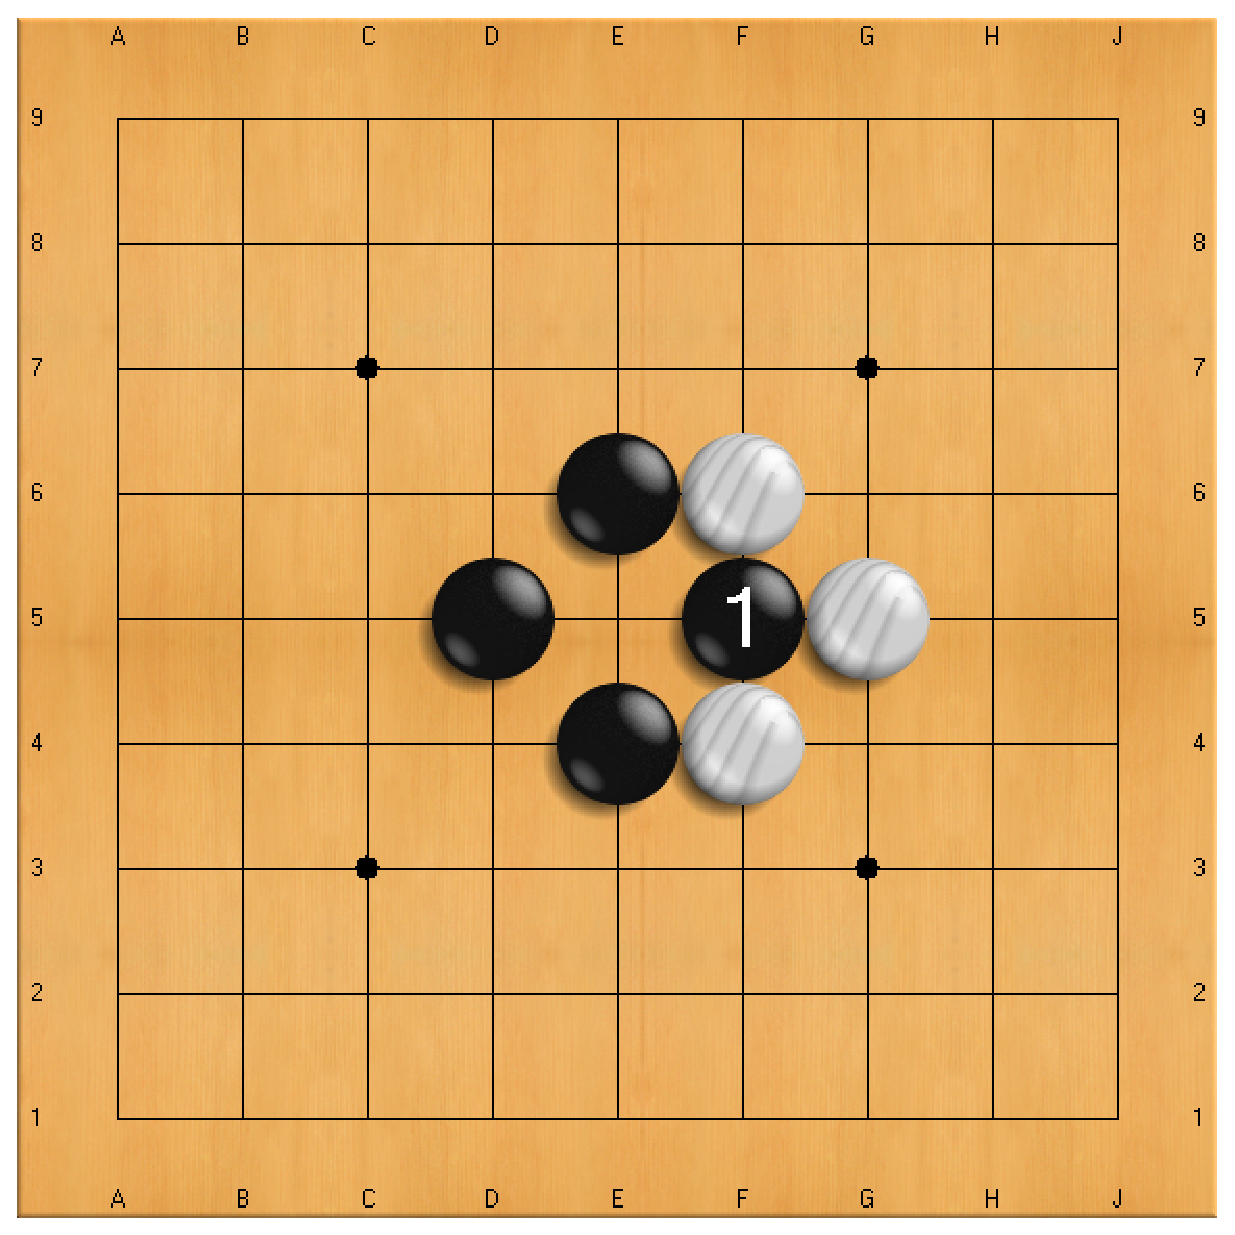
\includegraphics[scale=0.2]{contenido/cap2/imagenes/ko2.eps}
	\end{minipage}
	\caption[Situación de \textit{Ko} en el Go]{Situación de \textit{Ko}.}
	\label{fig:go_ko}
\end{figure}
\end{itemize}

Una partida de Go termina cuando ambos jugadores consideran que ya no existen territorios por disputar.
Cuando esto ocurre ambos jugadores pasan turno consecutivamente.
En una partida profesional, tal circunstancia la decide un juez.
Una partida también puede terminar si ambos jugadores han agotado sus piedras.

El \textbf{territorio} está formado por las intersecciones del tablero que se encuentren vacías.
El \textbf{territorio privado} está formado por las intersecciones que se encuentran dentro de algún cerco de uno u otro jugador.
El \textbf{territorio público} es aquel que no está cercado por ninguno de los jugadores y no influye en la puntuación final.
Hay ciertos territorios conquistados que no se encuentran protegidos del todo, pero que si el jugador contrario los atacase perdería de todas formas, luego son parte del territorio privado de quien lo tiene cercado.

El ganador de la partida es el jugador con más puntos.

\subsubsection{Puntuación}
\label{sssec:puntuacion_go}
Existen dos formas de contar los puntos de una partida: según las reglas japonesas y según las reglas chinas:

\bigskip

\begin{itemize}
	\item \textbf{Reglas japonesas}\\
	Cada jugador recibe un punto por cada intersección vacía dentro de su territorio, menos un punto por cada piedra que haya capturado el enemigo.
	\item \textbf{Reglas chinas}\\
	Cada jugador recibe un punto por cada intersección vacía dentro de su territorio, más un punto por cada piedra que tenga sobre el tablero. 
\end{itemize}
Ambos métodos producen el mismo resultado. Las reglas de puntuación japonesas son las más extendidas y son las que se usan en los torneos oficiales.

El jugador con piedras negras tiene ventaja debido a que siempre mueve primero.
Para compensar esta ventaja se suma una cantidad de puntos al jugador blanco.
A estos puntos se les denomina \textit{komi} y son determinados antes de empezar la partida.
El valor de \textit{komi} puede variar según los distintos reglamentos; suele oscilar entre 5.5 y 7.5 puntos para un tablero 19x19.
Este valor también es usado para evitar que una partida termine en empate.

\subsubsection{\textit{Handicap}}
\label{ssec:handicap_go}
En el Go existe un sistema de \textit{handicap} o ventaja para igualar una partida entre jugadores de diferente nivel.

El \textit{handicap} consiste en un número de piedras colocadas sobre el tablero antes de empezar la partida.
En ese caso el jugador de menor nivel jugará con las piedras negras y comenzará con un número determinado de piedras ya colocadas sobre el tablero.
Estas piedras se colocan sobre los puntos marcados del tablero, quedando las piedras de forma simétrica.
También existen otras variantes de \textit{handicap} libre, en el cual el jugador coloca las piedras de ventaja donde él quiera.

El número de piedras de \textit{handicap} depende de la diferencia de nivel entre los jugadores. 
Existe una clasificación oficial de niveles para los jugadores de Go \citeref{MCTS2}.







